\documentclass[conference]{IEEEtran}
\usepackage{graphicx}
\usepackage{url}
\usepackage{amsmath}
\usepackage[hidelinks]{hyperref}
\usepackage[sort&compress,comma,square,numbers]{natbib}

\begin{document}

\title{\vspace{10pt}Long-Horizon and Multi-Horizon Deep Learning for Great Lakes Water-Level Forecasting}

\author{
\IEEEauthorblockN{Alexander Stinnett}
\IEEEauthorblockA{
Michigan Technological University, Computer Science
}
\IEEEauthorblockN{Timothy C.~Havens}
\IEEEauthorblockA{
Michigan Technological University, Computer Science
}
\IEEEauthorblockN{Pengfei Xue}
\IEEEauthorblockA{
Michigan Technological University, Civil, Environmental, and Geospatial Engineering
}
}

\maketitle

\begin{abstract}

Great Lakes water levels affect infrastructure, navigation, and shoreline management, all of which benefit from planning in advance. Deep learning (DL) models have been used to predict Great Lakes water levels, but long-horizon forecasting remains challenging because hydroclimatic processes accumulate over time. This work systematically evaluated DL models for Lake Superior water-level forecasting across input representations, historical context lengths, forecast horizons ranging from 30 to 180 days ahead, and sequence-to-one predictions versus sequence-to-sequence predictions. Hyperparameter optimization (HPO) was employed within each condition, and configurations were selected using validation RMSE. Experiments showed that the validation-selected input representation and context length differed across sequence-to-one architectures, while the overall validation-selected 180-day configuration achieved a test RMSE of 12.2 cm. The sequence-to-sequence model was comparable in overall performance to multiple sequence-to-one models, with a mean horizon-wise relative RMSE difference of 0.82\% in favor of the sequence-to-sequence model. The sequence-to-sequence model had a 15.66\% higher test RMSE than the sequence-to-one model at the 30-day horizon, while the sequence-to-sequence model had lower test RMSE values across longer horizons from 90 to 180 days ahead. Selected models were refit across ten independent seeds and evaluated across threshold-based water-level regimes to assess robustness. The sequence-to-sequence model achieved lower test RMSE for all water-level regimes at longer horizons (120--180 days). In conclusion, in this Lake Superior evaluation, long-horizon forecasting performance depends not only on architecture but the entirety of the forecasting problem formulation, and multi-horizon forecasting models show comparable performance to multiple sequence-to-one models, which could reduce the number of experimental conditions in future works.


\end{abstract}


\section{Introduction}

The water levels of the Great Lakes affect coastal flooding, shoreline infrastructure, commercial navigation, and ecosystems \cite{fry2020operational}. Seasonal forecasts extending up to six months ahead are useful because many decisions require sufficient lead time for planning and preparation \cite{fry2020operational}. The U.S. Army Corps of Engineers (USACE), in coordination with Environment and Climate Change Canada, produces forecasts of monthly mean Great Lakes water levels up to six months ahead \cite{fry2020operational}. These forecasts provide expected lake-wide average water levels along with a range of possible levels under different future weather conditions \cite{fry2020operational}.

Long-horizon water-level prediction is difficult because Great Lakes water levels depend on interacting hydroclimatic processes such as precipitation, runoff, and evaporation, whose effects accumulate over seasonal timescales \cite{fry2020operational,barzegar2026interpretable,chen2025dualtransformer}. This makes both the amount of historical information and the way that information is represented important for seasonal forecasting.

Previous works have investigated historical water-level lags, preprocessing methods, atmospheric covariates, hyperparameter optimization (HPO), and horizon-specific seasonal forecasting \cite{wang2020lakeerie,kurt2024greatlakes,barzegar2021cnn,barzegar2026interpretable,chen2025dualtransformer}. However, these studies do not establish how different input representations and historical context lengths interact with model architecture, nor do they directly compare independently trained horizon-specific models with a joint multi-horizon output formulation under the same experimental framework. Seasonal prediction has also more commonly been formulated using separate horizon-specific models rather than directly comparing this approach against a single multi-output model.

This work evaluates multiple deep learning (DL) architectures, input representations, historical context lengths, and output formulations for seasonal water-level forecasting using Lake Superior as the focus. HPO was conducted within each condition using a separate validation period, and model configurations were selected using validation RMSE before evaluation on a held-out test period. The first analysis evaluates how input representation and historical context differ across DL architectures. The second compares six independently optimized horizon-specific models with a single joint multi-horizon model for forecasts from 30 to 180 days. Finally, the selected configurations are evaluated across multiple random initializations and water-level-change regimes. An open-source implementation of the experimental and evaluation framework is available in the
\href{https://github.com/Alexander-Stinnett/oceans-2026-great-lakes-water-level-forecasting}{\underline{GitHub repository}}.

\section{Related Work}

Wang \& Wang (2020) \cite{wang2020lakeerie} was an early example of Great Lakes machine learning (ML) prediction using daily Lake Erie water-level and meteorological data. Their study focused on short-horizon prediction. Kurt (2024) \cite{kurt2024greatlakes} performed monthly Great Lakes prediction but evaluated only one-month-ahead predictions. Barzegar (2021) \cite{barzegar2021cnn} used explicit multi-step monthly DL forecasting, but trained separate models for 1-, 2-, and 3-month-ahead targets using CNN-LSTM and wavelet preprocessing. Barzegar (2026) \cite{barzegar2026interpretable} used environmental-lag modeling and HPO, but focused on explaining environmental drivers of water-level variability instead of optimizing fixed-horizon forecasting accuracy. Chen (2025) \cite{chen2025dualtransformer} is the closest framework to this study because it targets forecasts up to six months ahead and uses the same Lake Superior data source. These studies demonstrate increasing use of temporal structure and environmental information, but they address different forecasting problems.

Barzegar (2021) \cite{barzegar2021cnn} used monthly water level without atmospheric covariates. The study trained ML/DL models on separate 1-, 2-, and 3-month-ahead targets and used Bayesian HPO with a 70/30 calibration-validation protocol. Chen (2025) \cite{chen2025dualtransformer} used the same Lake Superior data source as this study and applied a 30-day moving average (MA) over the input features. Their ``Prophet'' model used 12 historical samples spaced 30 days apart, while the ``Critic'' model used five future atmospheric samples between the forecast issue time and target. The ``Critic'' was therefore supplied with future atmospheric information from the reanalysis dataset, which would require forecasts of these atmospheric variables in an operational setting \cite{chen2025dualtransformer}. The study did not use HPO and instead used fixed hyperparameters for the tested models.

Chen (2025) reported an RMSE of 4.2 cm for 180-day-ahead Lake Superior water-level forecasting \cite{chen2025dualtransformer}. However, this result used future atmospheric information leading up to the forecast target, including atmospheric values up to 30 days before the target. The reported 4.2 cm RMSE therefore represents a different forecasting formulation from one restricted to information available at forecast origin. Their ablation results also show the importance of atmospheric information. In particular, substituting precipitation with its long-term mean increased RMSE from 4.2 cm to 9.4 cm \cite{chen2025dualtransformer}.


Prior work has shown that historical water-level lags, preprocessing, atmospheric covariates, and horizon-specific seasonal forecasting can affect prediction accuracy. However, these studies do not establish how multiple input representations and historical context lengths interact with model architecture, nor do they directly compare independently optimized horizon-specific sequence-to-one (seq2one) models with a joint sequence-to-sequence (seq2seq) multi-horizon formulation under a common experimental framework.

This study addresses several questions that remain unresolved by prior work. How should historical data be represented, and how much historical context should be used for seasonal forecasting? Does the preferred representation or context length depend on model architecture? Is it better to train six horizon-specific seq2one models or one joint seq2seq model? Finally, do the selected models remain robust across different random initializations and water-level-change regimes?


\section{Data and Methodology}

\subsection{Dataset and Preprocessing}

This work uses the Lake Superior dataset introduced in the Dual Transformer study \cite{chen2025dualtransformer}. The dataset contains seven daily variables spanning 1981--2023, with 15,705 observations before preprocessing. In the previous work, the first 29 samples were discarded to apply a 30-day causal MA over all features. In this work, the first 179 samples were discarded to utilize 30-, 60-, 90-, 120-, 150-, and 180-day MAs during exploratory experimentation, although selected input variants only included 30-day MAs.

The previous work also constructed datasets for Lake Michigan-Huron and Lake Erie, but this study focuses only on Lake Superior. The forecasting target is lake water level with a 30-day trailing MA applied. Past water level is included as an autoregressive input. The latest input observation occurs at forecast origin $t$, while the forecast target occurs at $t+h$. No observations after $t$ are included in the input. Lake water-level observations were derived from the coordinated network of U.S. and Canadian Great Lakes water-level gauges \cite{noaa2026waterlevels,usace2026waterlevels}.

Six spatially averaged exogenous variables describing atmospheric and lake conditions were used as predictors. Table~\ref{tab:dataset_variables} summarizes the variables, spatial domains, units, and data sources.

\begin{table}[t]
    \centering
    \caption{Lake Superior exogenous predictor variables and data sources.}
    \label{tab:dataset_variables}
    \small
    \begin{tabular}{llll}
    \hline
    \textbf{Variable} & \textbf{Domain} & \textbf{Unit} & \textbf{Source} \\
    \hline
    Air temperature & Lake      & $^\circ$C & CFSR/CFSv2 \\
    Air temperature & Watershed & $^\circ$C & CFSR/CFSv2 \\
    Wind speed      & Lake      & m/s       & CFSR/CFSv2 \\
    Wind speed      & Watershed & m/s       & CFSR/CFSv2 \\
    Precipitation   & Basin     & mm/day    & CFSR/CFSv2 \\
    LST             & Lake      & $^\circ$C & GLSEA$^{*}$ \\
    \hline
    \end{tabular}
    \par\vspace{1mm}
    \parbox{\columnwidth}{
        \footnotesize
        $^{*}$LST from 1981--1994 was obtained from the reconstructed data set of Kayastha et al.; GLSEA was used from 1995 onward.
    }
\end{table}

All exogenous variables except lake surface temperature (LST) were sourced from the Climate Forecast System Reanalysis (CFSR) \cite{saha2010cfsr}, covering January 1979 through March 2011, concatenated with the Climate Forecast System Version 2 (CFSv2) analysis product \cite{saha2014cfsv2} available from 2011 onward. LST data were sourced from the Great Lakes Surface Environmental Analysis (GLSEA) produced by the National Oceanic and Atmospheric Administration (NOAA) Great Lakes Environmental Research Laboratory (GLERL) \cite{noaa2026glsea}. Because GLSEA data are available only from 1995 onward, LST values from 1981--1994 were obtained from the reconstructed LST dataset developed using an LSTM model by Kayastha et al. (2023) \cite{kayastha2023lst}.

A 7:1:2 chronological split was used for training, validation, and testing. After removal of the first 179 samples, the target-date ranges were: training from June 29, 1981 through March 31, 2011; validation from April 1, 2011 through June 30, 2015; and testing from July 1, 2015 through December 31, 2023. Split membership was determined by target date.

Three input variants were evaluated: \emph{daily raw exogenous}, \emph{daily smoothed}, and \emph{sparse smoothed}. Daily raw exogenous inputs retain the 30-day MA water-level target while using raw daily exogenous observations at every time step in the context window. Daily smoothed inputs apply a 30-day MA to all features while retaining every daily time step. Sparse smoothed inputs also apply a 30-day MA to all features but sample one observation every 30 days. All transformations were causal and used only observations available at or before the forecast origin. No future atmospheric observations were provided to the models.

\begin{figure*}[!t]
\centering
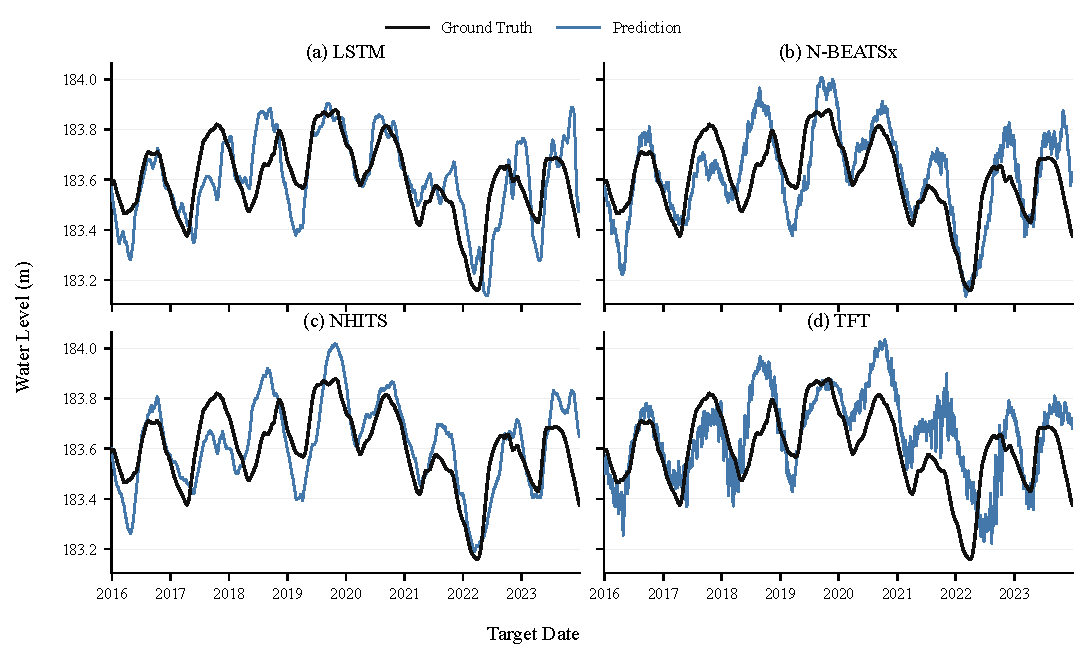
\includegraphics[
    height=0.35\textheight,
    keepaspectratio
]{figures/rq1_seq2one_180d_test_predictions_styled_wip.pdf}
\caption{Observed Lake Superior water levels and 180-day-ahead predictions from the validation-selected (a) LSTM, (b) N-BEATSx, (c) NHITS, and (d) TFT configurations over the test period.}
\label{fig:seq2one_180d_predictions}
\end{figure*}


\subsection{Forecasting Formulations}

Let $t$ denote the forecast origin and $\tilde{y}_t$ denote the 30-day trailing MA water level at time $t$. The configured historical context lengths were $C \in \{180,360,540,720\}$ days. For the sparse smoothed input, these settings correspond to $N_C \in \{6,12,18,24\}$ observations sampled at 30-day intervals. The model input is denoted as $\mathbf{X}_t^{(v,C)}$, where $v$ represents the input variant and $C$ represents the configured context length.

Forecast horizons were defined as
\[
    \mathcal{H}=\{30,60,90,120,150,180\}\text{ days}.
\]
All targets remain daily indexed and represent the 30-day trailing MA water level rather than calendar-month observations.

Two output formulations were evaluated: seq2one and seq2seq. Seq2one predicts one target at a specified forecast horizon:
\[
    f_h\left(\mathbf{X}_t^{(v,C)}\right)
    \rightarrow
    \tilde{y}_{t+h},
    \qquad h \in \mathcal{H}.
\]

The seq2seq formulation jointly predicts all six forecast horizons:
\[
    f\left(\mathbf{X}_t^{(v,C)}\right)
    \rightarrow
    \left[
    \tilde{y}_{t+30},
    \tilde{y}_{t+60},
    \tilde{y}_{t+90},
    \tilde{y}_{t+120},
    \tilde{y}_{t+150},
    \tilde{y}_{t+180}
    \right].
\]


\subsection{Deep Learning Models}

Four DL architectures were evaluated using the NeuralForecast Python package \cite{olivares2022neuralforecast}: Long Short-Term Memory (LSTM), Neural Basis Expansion Analysis with Exogenous Variables (N-BEATSx), Neural Hierarchical Interpolation for Time Series Forecasting (NHITS), and Temporal Fusion Transformer (TFT). These architectures support exogenous inputs and represent recurrent, basis-expansion, hierarchical-interpolation, and attention-based forecasting approaches, respectively \cite{hochreiter1997lstm,olivares2023nbeatsx,challu2023nhits,lim2021tft}. Each architecture was evaluated over the same input variants, context settings, and forecasting formulations using mean squared error (MSE) loss.


\subsection{Hyperparameter Optimization and Evaluation}

A separate validation split and HPO procedure were used for systematic model selection. The experimental grid contained four architectures, four context settings, three input variants, and seven forecasting formulations---six seq2one horizons and one six-output seq2seq formulation---for a total of 336 conditions.

Optuna \cite{akiba2019optuna} was used to optimize each condition independently, with 50 successful trials completed per condition. Learning rate, batch size, windows batch size, dropout, and architecture-specific width, depth, and structural parameters were tuned. Standard scaling was fixed across experiments and was not included in the search space.

Each Optuna trial was trained for 750 optimizer updates using MSE loss, with validation RMSE as the optimization objective. For seq2seq conditions, the objective was one RMSE calculated across all six outputs and validation samples. The Tree-structured Parzen Estimator (TPE) sampler \cite{bergstra2011tpe} was used for hyperparameter selection. The \texttt{constant\_liar=True} setting was used to discourage redundant suggestions when multiple workers accessed the same Optuna study.

Within each condition, the trial with the lowest Optuna validation objective was retained. Cross-condition comparisons were then based on the selection RMSE of each retained configuration on the validation set. Selected configurations were refit from scratch using the combined training and validation sets with the same 750-update training budget before final test evaluation.

Final test comparisons were restricted to 2,926 common forecast origins from July 1, 2015 through July 4, 2023. This ensured that every forecast originated after the training and validation period and that the complete 180-day seq2seq target block was available for every origin. Seq2one, seq2seq, and persistence comparisons therefore used identical forecast origins.


\subsection{Robustness Evaluation}

For the regime analysis, the six validation-selected horizon-specific seq2one configurations and the single validation-selected seq2seq configuration were each independently refit using ten seeds. Hyperparameters remained fixed, and every refit used the combined training and validation data. No additional HPO or post-refit model selection was performed.

Water-level regimes were defined using horizon-specific changes in the 30-day MA target. For each horizon $h$,
\[
    \Delta \tilde{y}_t^{(h)}
    =
    \tilde{y}_{t+h}-\tilde{y}_t.
\]

Let $q_{1/3}^{(h)}$ and $q_{2/3}^{(h)}$ denote the lower and upper terciles of $\Delta \tilde{y}_t^{(h)}$ over the combined training and validation period. Regime membership was defined as
\[
    R_t^{(h)} =
    \begin{cases}
    \text{Falling}, & \Delta \tilde{y}_t^{(h)} < q_{1/3}^{(h)}, \\[4pt]
    \text{Stable}, & q_{1/3}^{(h)} \le \Delta \tilde{y}_t^{(h)} \le q_{2/3}^{(h)}, \\[4pt]
    \text{Rising}, & \Delta \tilde{y}_t^{(h)} > q_{2/3}^{(h)}.
    \end{cases}
\]

Thresholds were estimated separately for each $h \in \mathcal{H}$ using only the combined training and validation period. They were then fixed before test evaluation and applied identically to all forecasting systems.

Persistence was included as a non-learned reference forecast \cite{hyndman2021forecasting}:
\[
    \hat{\tilde{y}}_{t+h} = \tilde{y}_t.
\]

Persistence and both neural forecasting formulations were evaluated over identical forecast origins within each horizon and regime. Neural-model RMSE values were summarized across the ten independent refits using the mean and sample standard deviation.


\section{Results}

\subsection{RQ1: Configuration Selection and 180-Day Forecasting}

RQ1 evaluates how the validation-selected input representation and historical context differ across architectures for 180-day-ahead seq2one forecasting, and how the selected configurations perform on the held-out test set. Table~\ref{tab:rq1_180d} summarizes the validation-selected 180-day configurations.

\begin{table}[htbp]
    \centering
    \caption{Validation-selected configurations for 180-day seq2one forecasting.}
    \label{tab:rq1_180d}
    \footnotesize
    \setlength{\tabcolsep}{6pt}
    \renewcommand{\arraystretch}{1.05}
        \begin{tabular}{@{}llccc@{}}
        \hline
        \textbf{Model} & \textbf{Input} & \textbf{Context} &
        \textbf{Selection RMSE} & \textbf{Test RMSE} \\
         & & \textbf{(days)} & \textbf{(cm)} & \textbf{(cm)} \\
        \hline
        LSTM     & Daily smooth.  & 540 & 9.55 & 12.84 \\
        N-BEATSx & Sparse smooth. & 720 & \textbf{8.88} & 12.20 \\
        NHITS    & Daily smooth.  & 720 & 9.03 & \textbf{12.03} \\
        TFT      & Sparse smooth. & 360 & 8.90 & 15.56 \\
        \hline
        \end{tabular}
\end{table}

The selected configuration differed by architecture. None of the four models selected the shortest 180-day context, with selected context lengths ranging from 360 to 720 days. LSTM and NHITS selected daily smoothed inputs, while N-BEATSx and TFT selected sparse smoothed inputs. N-BEATSx and NHITS both used the longest configured context of 720 days. N-BEATSx had the lowest selection RMSE at 8.88 cm, narrowly below TFT at 8.90 cm. However, TFT produced the highest test RMSE at 15.56 cm.

Figure~\ref{fig:seq2one_180d_predictions} shows the 180-day-ahead predictions from the selected configuration of each DL architecture. All four models capture the broad rising and falling water-level patterns at this long forecast horizon. Larger errors are visible during some periods of more rapid change, with the magnitude of these errors differing by architecture.

Overall, the 180-day results show that the selected input representation and historical context are architecture-dependent. NHITS achieved the lowest test RMSE at 12.03 cm, followed by N-BEATSx at 12.20 cm. TFT had the highest test RMSE despite having a selection RMSE close to the lowest value.


\subsection{RQ2: Multi-Horizon Forecasting}

RQ2 evaluates the accuracy tradeoff between independently optimized horizon-specific seq2one models and a single six-output seq2seq model across 30- to 180-day forecast horizons. The selected seq2one model for each horizon was compared with the single selected seq2seq model. The relative difference in test RMSE is defined as

\[
    \Delta_{\mathrm{RMSE},h} =
    100\left(
    \frac{\mathrm{RMSE}_{\mathrm{seq2seq},h}}
    {\mathrm{RMSE}_{\mathrm{seq2one},h}}
    -1
    \right).
\]

A positive value indicates lower RMSE for seq2one, while a negative value indicates lower RMSE for seq2seq. The selected seq2seq model was NHITS using daily raw exogenous inputs and 540 days of configured context. Table~\ref{tab:rq2_multihorizon} reports the horizon-wise test comparison.

\begin{table}[htbp]
\centering
\caption{Test RMSE comparison between validation-selected seq2one models and the single validation-selected seq2seq model.}
\label{tab:rq2_multihorizon}
\small
\setlength{\tabcolsep}{4pt}
    \begin{tabular}{@{}ccccc@{}}
    \hline
    \textbf{Horizon} &
    \textbf{Seq2one} &
    \textbf{Seq2one} &
    \textbf{Seq2seq} &
    \textbf{$\Delta$ RMSE$_h$} \\
    \textbf{(days)} &
    \textbf{Model} &
    \textbf{RMSE (cm)} &
    \textbf{RMSE (cm)} &
    \textbf{(\%)} \\
    \hline
    30  & TFT       & \textbf{3.75} & 4.34 & +15.66 \\
    60  & LSTM      & \textbf{6.55} & 6.78 & +3.61  \\
    90  & TFT       & 9.05 & \textbf{8.46} & -6.54  \\
    120 & LSTM      & 10.38 & \textbf{9.49} & -8.61 \\
    150 & TFT       & 10.81 & \textbf{10.40} & -3.76 \\
    180 & N-BEATSx  & 12.20 & \textbf{11.56} & -5.28 \\
    \hline
    \end{tabular}
\end{table}

\begin{table*}[!t]
    \centering
    \caption{Test RMSE across water-level regimes for the validation-selected seq2one models, the validation-selected seq2seq model, and persistence. Neural-model values report the mean $\pm$ sample standard deviation across ten independent refits.}
    \label{tab:rq3_regime_rmse}
    \small
    \setlength{\tabcolsep}{7pt}
    \begin{tabular}{@{}ccccc@{}}
        \hline
        \textbf{Horizon} &
        \textbf{Regime} &
        \textbf{Seq2one RMSE} &
        \textbf{Seq2seq RMSE} &
        \textbf{Persistence RMSE} \\
        \textbf{(days)} &
        &
        \textbf{(cm)} &
        \textbf{(cm)} &
        \textbf{(cm)} \\
        \hline

        30  & Falling & $\mathbf{3.18 \pm 0.21}$ & $3.97 \pm 0.32$ & $6.67$ \\
        30  & Stable  & $\mathbf{3.45 \pm 0.40}$ & $3.86 \pm 0.24$ & $2.06$ \\
        30  & Rising  & $\mathbf{4.78 \pm 0.29}$ & $5.15 \pm 0.16$ & $9.19$ \\
        \hline

        60  & Falling & $6.40 \pm 0.73$ & $\mathbf{5.79 \pm 0.34}$ & $12.14$ \\
        60  & Stable  & $\mathbf{5.83 \pm 0.56}$ & $5.90 \pm 0.29$ & $4.06$ \\
        60  & Rising  & $\mathbf{8.02 \pm 0.57}$ & $8.26 \pm 0.35$ & $16.00$ \\
        \hline

        90  & Falling & $\mathbf{6.72 \pm 0.94}$ & $6.73 \pm 0.34$ & $17.44$ \\
        90  & Stable  & $8.88 \pm 1.23$ & $\mathbf{8.51 \pm 0.29}$ & $6.34$ \\
        90  & Rising  & $10.54 \pm 0.80$ & $\mathbf{9.54 \pm 0.57}$ & $20.96$ \\
        \hline

        120 & Falling & $8.49 \pm 0.82$ & $\mathbf{8.20 \pm 0.51}$ & $21.59$ \\
        120 & Stable  & $10.89 \pm 0.65$ & $\mathbf{9.88 \pm 0.37}$ & $7.61$ \\
        120 & Rising  & $11.73 \pm 0.85$ & $\mathbf{10.39 \pm 0.67}$ & $24.28$ \\
        \hline

        150 & Falling & $10.75 \pm 1.08$ & $\mathbf{9.58 \pm 0.55}$ & $23.88$ \\
        150 & Stable  & $12.20 \pm 1.14$ & $\mathbf{11.15 \pm 0.52}$ & $7.66$ \\
        150 & Rising  & $12.42 \pm 1.22$ & $\mathbf{10.93 \pm 0.69}$ & $26.22$ \\
        \hline

        180 & Falling & $11.08 \pm 0.29$ & $\mathbf{10.65 \pm 0.51}$ & $25.69$ \\
        180 & Stable  & $13.23 \pm 0.45$ & $\mathbf{12.46 \pm 0.62}$ & $7.68$ \\
        180 & Rising  & $12.16 \pm 0.33$ & $\mathbf{11.91 \pm 0.87}$ & $27.37$ \\
        \hline
    \end{tabular}
\end{table*}

The seq2one models had lower test RMSE at 30 and 60 days, while the seq2seq model had lower RMSE at every horizon from 90 to 180 days. At 30 days, seq2seq had 15.66\% higher RMSE than seq2one. At 60 days, the difference decreased to 3.61\%. Across all six horizons, the arithmetic mean of the horizon-specific relative RMSE differences was $-0.82\%$, corresponding to an average reduction of 0.82\% for seq2seq under this summary. Therefore, the single multi-output model provided comparable overall accuracy to six independently optimized horizon-specific models while producing lower RMSE at the four longest horizons.

\subsection{RQ3: Robustness Analysis}

RQ3 evaluates how robust the selected forecasting models are across water-level regimes and random initialization. As described in the methodology, the selected seq2one and seq2seq configurations were independently refit using ten seeds, and the same regime thresholds were applied to all forecasting systems. Table~\ref{tab:rq3_regime_rmse} reports test RMSE across the water-level regimes.

Persistence had its lowest RMSE in the stable regime at every horizon and had lower RMSE than both neural systems in all six stable-regime comparisons. In contrast, both neural systems outperformed persistence in every falling and rising regime. The difference between the neural models and persistence was especially large at the longer horizons.

The relative performance of seq2one and seq2seq also changed with horizon. Seq2one had lower mean RMSE in all three regimes at 30 days. At 60 days, seq2seq performed better in the falling regime, while seq2one performed better in the stable and rising regimes. At 90 days, seq2one was slightly better in the falling regime, while seq2seq was better in the stable and rising regimes. From 120 through 180 days, seq2seq had lower mean RMSE in all three regimes. This follows the same general pattern as RQ2, where seq2one performed better at shorter horizons and seq2seq performed better at the longer horizons.

Across the 18 horizon--regime combinations, the sample standard deviation across ten refits ranged from 0.21 to 1.23 cm for seq2one and from 0.16 to 0.87 cm for seq2seq. The selected seq2seq model therefore had lower seed-to-seed variability on average, although this was not true for every horizon and regime.

Overall, the selected models had relatively small variation across independent refits, while their relative accuracy depended on forecast horizon and water-level regime. Learned forecasting provided the largest advantage over persistence during rising and falling conditions, and seq2seq had lower mean RMSE across all three regimes at the longest horizons.


\section{Discussion}

Among the selected 180-day seq2one models, no single input representation was favored across all architectures. None selected the daily raw exogenous variant. None of the selected configurations used the shortest 180-day context either, with selected context lengths ranging from 360 to 720 days. This shows that selection for the 180-day forecasting task favored longer contexts, while the preferred input representation depended on architecture.

The validation and test rankings were also not identical. The selected seq2seq model also used a different configuration from the selected 180-day seq2one models. This further shows that the preferred configuration depended on both architecture and forecasting task.

The seq2one and seq2seq comparison also depended on forecast horizon. Seq2one had lower test RMSE at 30 and 60 days, while seq2seq had lower test RMSE at every horizon from 90 through 180 days. Therefore, independently optimized horizon-specific models do not necessarily give better long-range forecasting accuracy than a jointly optimized multi-horizon model. Using seq2seq also reduces the number of independent optimization problems needed to cover multiple forecast horizons, which provides a useful accuracy-to-optimization tradeoff for medium- to long-horizon forecasting.

The robustness analysis showed a similar horizon-dependent pattern. Persistence had lower RMSE than both neural systems in every stable regime, while both neural systems had lower RMSE than persistence in every falling and rising regime. The longer-horizon advantage seen in RQ2 therefore also appeared across the regime-based evaluation.

The selected seq2seq configuration also had lower seed-to-seed variability on average. Across all horizon--regime combinations, the mean standard deviation was approximately 0.46 cm for seq2seq and 0.70 cm for the horizon-specific seq2one models. At 180 days, the seq2one configuration had lower standard deviation than seq2seq in all three regimes.

Compared with Chen et al. \cite{chen2025dualtransformer}, the models in this study do not use future atmospheric observations that would be unavailable at forecast origin. Chen et al. reported a 180-day-ahead RMSE as low as 4.2 cm, but their ``Critic'' formulation used future atmospheric information extending toward the forecast target. Their evaluation also used a substantially shorter test period, while this study used a separate validation period for model selection and evaluated the final forecasts over approximately eight years of common test forecast origins. These differences in available information, validation procedure, and evaluation design mean that the RMSE values represent different forecasting problems and should not be treated as direct model-to-model performance comparisons.

This study extends prior Great Lakes forecasting work by evaluating input representation, historical context, architecture, and seq2one versus seq2seq output formulations under the same experimental framework. It also evaluates robustness across random initialization and different water-level-change regimes over multiple forecast horizons.

Several limitations remain. This study focuses only on Lake Superior, although comparable data are available for other Great Lakes systems. The HPO search spaces and input variants evaluated here represent only a finite set of possible configurations and do not guarantee globally optimal forecasting performance. The models also produce deterministic forecasts and do not explicitly represent predictive uncertainty by using a probabilistic output.


\section{Conclusion}

This work evaluated multiple DL architectures, input representations, context lengths, and output formulations for Lake Superior water-level forecasting using HPO and validation-based model selection. Seq2one models were optimized independently for horizons from 30 to 180 days and compared with a single six-output seq2seq model.

The selected configurations depended on architecture and forecasting task, and no single input representation or context length was selected across all of the validation-selected models. Seq2one had lower test RMSE at 30 and 60 days, while the selected seq2seq model had lower test RMSE at every horizon from 90 through 180 days. In the robustness analysis, seq2seq also had lower mean RMSE in all three water-level regimes from 120 through 180 days. Both neural systems outperformed persistence in all rising and falling regime comparisons, while persistence had lower RMSE than both neural systems in the stable regimes.

The relative performance of seq2one and seq2seq also changed with horizon. Seq2one had lower mean RMSE in all three regimes at 30 days, while the intermediate horizons were mixed. From 120 through 180 days, seq2seq had lower mean RMSE in all three regimes, following the same general horizon-dependent pattern as RQ2. The results also show that input representation and historical context should not be assumed to transfer across architectures or forecasting tasks. The models in this study use only information available at or before forecast origin and do not rely on future atmospheric observations.

Reported RMSE values should be interpreted according to the forecasting problem being evaluated. The results in this work are numerically better than those reported in some previous Great Lakes forecasting studies such as Barzegar et al. \cite{barzegar2021cnn}, while the lowest errors reported by Chen et al. \cite{chen2025dualtransformer} are lower than those obtained here. However, these studies differ in forecast targets, available predictors, forecast horizons, and evaluation procedures. In particular, Chen et al. used future atmospheric information, while the models in this study use only historically available observations.

Future work can extend this framework to the other Great Lakes datasets available from Chen et al. \cite{chen2025dualtransformer}, evaluate probabilistic forecasting to represent predictive uncertainty, and develop continuously updated data pipelines for repeated model training as new atmospheric and hydrologic observations become available.


\section*{Acknowledgments}

OpenAI ChatGPT (GPT-5.6 Sol) was used to assist with drafting and grammar throughout the manuscript, including generating and restructuring text from author-provided technical content. Codex assisted extensively with software implementation, refactoring, debugging, and documentation. The authors defined the research methodology, experimental design, analyses, and scientific interpretations and reviewed, tested, and validated all AI-assisted text and software.

This material is based upon work supported by the National Science Foundation under Grant Number 2244403 and Grant Number 2438826.

\newpage

\bibliographystyle{IEEEtran}
\bibliography{references}

\end{document}
